\subsubsection{Stéganographie dans le domaine transformé\cite{DWT-DCT,Ondelettes}}

\paragraph{Introduction}~\\\indent
Cette technique de stéganographie consiste à intégrer l'information secrète dans un domaine transformé du signal. Dans une image, on distingue le domaine spatial, basé sur les pixels, et son domaine transformé qui est celui des fréquences. Les techniques de stéganographie sur le domaine transformé utilisent la transformée orhtognale de l'image (exemple : transformée de Fourier discrète) plutôt que l'image elle-même. La transformée orthogonale ayant donc deux composantes, la magnitude et la phase.\\

Nous ne présentons ici qu'une des méthodes utilisées dans le domaine transformé : l'utilisation de la transformée d'ondelettes discrète (DWT, pour \emph{Discrete Wavelet Transform}).

\paragraph{Transformée d'ondelettes discrète (DWT)}~\\\indent
La DWT permet une décomposition hiérarchique d'une image. Elle se base sur l'utilisation d'ondelettes qui sont de fréquences et durées variables. Ces ondelettes permettent à la fois une description spatiale et fréquentielle de l'image : la DWT indique quelle fréquence apparaît, où, et sur quelle surface. La transformée en ondelettes détecte les zones riches en informations (à fort contraste) et les sépare. Une ondelette est une fonction de valeur moyenne nulle et limitée dans le temps. Les ondelettes sont générées par des translations, compressions et dilatations d'une ondelette mère. \\

L'application de la DWT, consiste à filtrer l'image dans les deux dimensions (filtrage vertical, horizontal et diagonal). Ces filtres décomposent l'image en 4 parties (sous-bandes) de résolution inférieure. Ces sous-bande sont sans chevauchement et ont différentes résolutions, on les nomme LL, LH, HL et HH. La sous-bande LL correspond aux coefficients de corrélation déterminés par une fonction d'ondelette dilatée jouant le même rôle qu'un filtre passe bas. Les autres sous bandes montrent les valeurs déterminées par la fonction d'ondelette mère compressée, faisant office de filtres passe haut. On peut appliquer plusieurs DWT à la suite, on le fait alors sur la sous-bande LL. Après $N$ DWT on se retrouve ainsi avec $3N+1$ sous-bandes.\\

Par sa capacité à bien représenter les fréquences dans l'espace, la DWT est très efficace pour la stéganographie. En effet, la plus grande quantité d'énergie dans l'image est stockée dans les basses fréquences (sous-bande LL$_{N}$). Ainsi, cacher un message en basse fréquence altérerait beaucoup la qualité de l'image et serait facilement décelable, même si cela serait plus robuste. Par conséquent, cacher un message dans les hautes fréquences (sous-bandes LH$_{X}$ et HL$_{X}$) serait bien plus discret car l'\oe il humain remarque difficilement les changements dans les contours.\\

\begin{figure}[h]
\centering
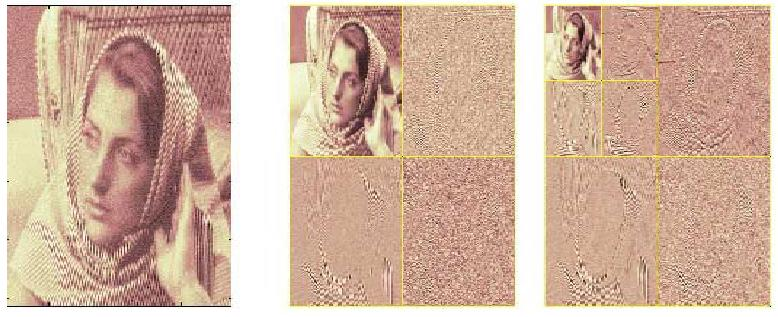
\includegraphics[width=\linewidth]{images/dwt-exemple.jpg}
\caption{Exemple de deux DWT successives (sur l'image du milieu : LL en haut à gauche, LH en bas à gauche, HL en haut à droite, HH en bas à droite)}
\end{figure}

\paragraph{Algorithme générique d'implantation et d'extraction d'un message}~\\\indent
\subparagraph{Implantation d'un message secret}
\begin{enumerate}
\item Étudier l'image et le message secret (texte/image) pour trouver la meilleure manière de le cacher.
\item Transformer le message en fichier binaire s'il ne l'est pas encore. Réaliser une DWT sur l'image de couverture.
\item Déterminer les coefficients de filtrage dans les directions verticale et horizontale (LH et HL). Cacher les bits du message dans ces coefficients (remplacement).
\item Créer la stego-image (par transformée inverse IDWT).
\end{enumerate}

\subparagraph{Extraction d'un message secret}
\begin{enumerate}
\item Étudier la stego-image pour savoir comment a pu être dissimulé le message.
\item Calculer la DWT et extraire les coefficients de filtrage verticaux et horizontaux.
\item Reconstruire le message bits par bits à partir des coefficients.
\item Recomposer le message compréhensible par l'humain.
\end{enumerate}

\begin{figure}[h]
	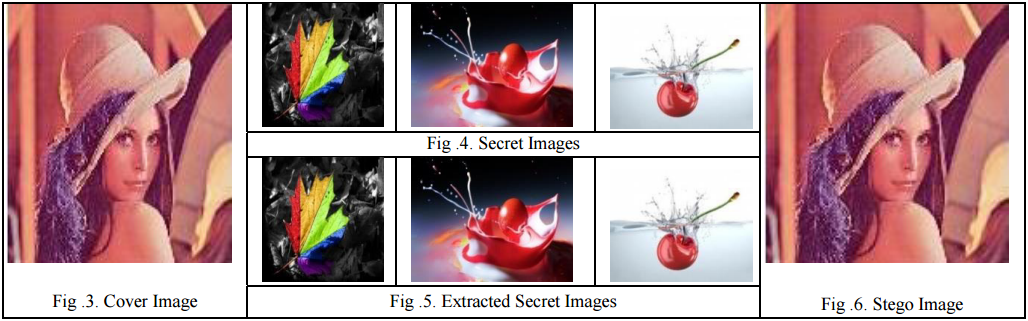
\includegraphics[width=\linewidth]{images/dwt-stego-exemple.png}
	\centering \caption{Exemple de stéganographie avec une DWT : implantation de trois images secrètes dans une seule en utilisant les trois canaux RGB\cite{DWT-RGB}}
\end{figure}

\paragraph{Commentaire}~\\\indent
La DWT est une des transformations les plus robustes et les plus efficaces pour la stéganographie dans le domaine transformé. Elle ne permet pas de cacher un gros volume de données mais assure une forte invisibilité du message, une forte robustesse contre les traitements d'image ultérieurs et permet une faible détérioration du message à l'extraction. Elle est souvent présentée comme la méthode la plus sûre pour la stéganographie dans le domaine transformé.